\documentclass[11pt,a4paper,twoside]{article}

% ============================================================================
% PAQUETES ESENCIALES
% ============================================================================
\usepackage[spanish]{babel}
\usepackage[margin=2.5cm]{geometry}
\usepackage{graphicx}
\usepackage{booktabs}
\usepackage{array}
\usepackage{multirow}
\usepackage{hyperref}
\usepackage{xcolor}
\usepackage{fancyhdr}
\usepackage{lastpage}
\usepackage{float}
\usepackage{amsmath}
\usepackage{amssymb}
\usepackage{tikz}
\usepackage{pgfplots}
\usepackage{listings}
\usepackage{xfrac}
\usepackage{caption}
\usepackage{subcaption}

% ============================================================================
% CONFIGURACIÓN DE COLORES Y ESTILOS
% ============================================================================
\definecolor{darkblue}{rgb}{0.0, 0.2, 0.6}
\definecolor{lightblue}{rgb}{0.0, 0.4, 0.8}
\definecolor{accent}{rgb}{1.0, 0.3, 0.0}
\definecolor{darkred}{rgb}{0.8, 0.0, 0.0}

\hypersetup{
    colorlinks=true,
    linkcolor=darkblue,
    urlcolor=lightblue,
    citecolor=darkblue
}

% ============================================================================
% ENCABEZADO Y PIE DE PÁGINA
% ============================================================================
\pagestyle{fancy}
\fancyhf{}
\fancyhead[LE,RO]{\textcolor{darkblue}{\textbf{People Analytics: FinanCorp Chile}}}
\fancyhead[LO,RE]{\small\textit{Diagnóstico de Rotación y Retención de Talento}}
\fancyfoot[LE,RO]{\thepage\ de \pageref{LastPage}}
\fancyfoot[LO,RE]{\small\textit{Mayo 2026}}
\renewcommand{\headrulewidth}{1.5pt}
\renewcommand{\footrulewidth}{0.5pt}

% ============================================================================
% CONFIGURACIÓN DE TÍTULOS Y SECCIONES
% ============================================================================
\usepackage{titlesec}

\titleformat{\section}
  {\normalfont\Large\bfseries\color{darkblue}}
  {\thesection}{1em}{}[\titlerule]

\titleformat{\subsection}
  {\normalfont\large\bfseries\color{lightblue}}
  {\thesubsection}{0.8em}{}

\titleformat{\subsubsection}
  {\normalfont\normalsize\bfseries\color{accent}}
  {\thesubsubsection}{0.6em}{}

% ============================================================================
% CONFIGURACIÓN DE FIGURAS Y TABLAS
% ============================================================================
\captionsetup{font=small, labelfont=bf, textfont=it}
\setlength{\parindent}{0em}
\setlength{\parskip}{0.5em}

% ============================================================================
% INICIO DEL DOCUMENTO
% ============================================================================
\begin{document}

% ============================================================================
% PORTADA
% ============================================================================
\thispagestyle{empty}
\begin{center}
    \vspace*{2cm}
    
    {\fontsize{28}{34}\selectfont\color{darkblue}\textbf{PEOPLE ANALYTICS}}
    
    \vspace{0.5cm}
    
    {\fontsize{18}{22}\selectfont\color{lightblue}\textbf{Diagnóstico de Rotación, Retención y Fuga de Talento}}
    
    \vspace{0.5cm}
    
    {\fontsize{14}{17}\selectfont\color{accent}\textit{FinanCorp Chile — Caso de Estudio}}
    
    \vspace{3cm}
    
    \begin{tikzpicture}
        \draw[darkblue, line width=0.5mm] (0,0) -- (15,0);
        \draw[lightblue, line width=0.3mm] (0,-0.3) -- (15,-0.3);
    \end{tikzpicture}
    
    \vspace{3cm}
    
    \begin{tabular}{ll}
        \textbf{Empresa:} & FinanCorp Chile (Caso Ficticio) \\
        \textbf{Dotación:} & 3,200 colaboradores \\
        \textbf{Rotación Actual:} & 22\% (\(\sim\)703 salidas anuales) \\
        \textbf{Costo de Rotación:} & USD \$2.109.000 anuales \\
        \textbf{Fecha de Análisis:} & 13 de mayo de 2026 \\[6pt]
        \multicolumn{2}{l}{\textcolor{darkblue}{\rule{10cm}{0.4pt}}} \\[4pt]
        \textbf{Integrantes:} & Daniel Avello \\
                              & Felipe Valdivia \\
                              & Roberto Sepúlveda \\
                              & Christofer Palominos \\
                              & José Luis Gajardo Angel \\
    \end{tabular}
    
    \vfill
    
    {\large\textbf{Análisis Predictivo basado en Machine Learning}}
    
    {\small\textit{Modelo: Regresión Logística (umbral óptimo 0.54) — ROC-AUC: 70.5\%}}
    
    \vspace{2cm}
\end{center}

\newpage

% ============================================================================
% RESUMEN EJECUTIVO
% ============================================================================
\section*{Resumen Ejecutivo}

Este análisis implementa un modelo analítico avanzado para identificar, explicar y anticipar la fuga de talento en organizaciones del sector financiero. Mediante técnicas de análisis exploratorio de datos, segmentación de riesgo y modelado predictivo con Machine Learning, se proporciona una base data-driven para decisiones estratégicas de retención de personal.

\subsection*{Hallazgos Clave}

\begin{itemize}
    \item \textbf{Rotación Crítica:} La rotación en áreas críticas (25.2\%) es \textbf{6.7 veces superior} a otras áreas (3.8\%)
    \item \textbf{Impacto Financiero:} Pérdida anual de USD \$2.109.000 en costos de reemplazo
    \item \textbf{Oportunidad:} Reducir rotación 15\% implicaría ahorrar USD \$316.350 anuales
    \item \textbf{Predicción Efectiva:} Modelo con 65.9\% de precisión predictiva (ROC-AUC)
    \item \textbf{Intervención Selectiva:} 79 personas en riesgo muy alto requieren atención inmediata
\end{itemize}

\subsection*{Recomendación Principal}

Implementar un programa de intervención en tres niveles con enfoque en las 79 personas clasificadas en riesgo muy alto, proyectando un impacto de USD \$1.671.500 en ahorro directo durante los primeros 3 años.

\newpage

% ============================================================================
% TABLA DE CONTENIDOS
% ============================================================================
\tableofcontents
\newpage

% ============================================================================
% SECCIÓN 1: INTRODUCCIÓN
% ============================================================================
\section{Introducción}

\subsection{Contexto y Problemática}

La rotación de personal representa uno de los mayores desafíos estratégicos para las organizaciones modernas. En el sector financiero, donde la continuidad operacional y la expertise son críticos, la fuga de talento genera impactos significativos en:

\begin{itemize}
    \item \textbf{Costos Directos:} Reclutamiento, selección y capacitación de nuevos colaboradores
    \item \textbf{Costos Indirectos:} Pérdida de productividad, disrupciones operacionales, impacto en clima
    \item \textbf{Riesgos Estratégicos:} Vulnerabilidad en áreas críticas, pérdida de conocimiento organizacional
    \item \textbf{Reputacionales:} Deterioro de marca empleadora, dificultad en atraer talento
\end{itemize}

FinanCorp Chile enfrenta una rotación del 22\% anual, significativamente por encima de la industria (15\%), generando una pérdida estimada de USD \$2.109.000 anuales. Esta situación requiere una intervención estratégica basada en datos.

\subsection{Objetivos del Análisis}

\begin{enumerate}
    \item Construir un modelo predictivo para identificar colaboradores en riesgo de rotación
    \item Explicar los factores determinantes en la decisión de abandono
    \item Priorizar intervenciones por impacto y urgencia
    \item Proporcionar recomendaciones estratégicas con ROI estimado
\end{enumerate}

\subsection{Metodología}

Este análisis combina técnicas de:

\begin{itemize}
    \item \textbf{Análisis Exploratorio:} Estadísticas descriptivas y correlaciones
    \item \textbf{Segmentación:} Clasificación de riesgo mediante scoring
    \item \textbf{Machine Learning:} Comparación de Regresión Logística vs. Random Forest
    \item \textbf{Análisis de Impacto:} Matriz de riesgo-urgencia y priorización
\end{itemize}

\newpage

% ============================================================================
% SECCIÓN 2: ANÁLISIS EXPLORATORIO DE DATOS (EDA)
% ============================================================================
\section{Análisis Exploratorio de Datos}

\subsection{Estadísticas Descriptivas}

El dataset contiene información de 3.200 colaboradores con 11 variables predictoras.

\textbf{Métricas Principales:}

\begin{table}[H]
    \centering
    \caption{Estadísticas Descriptivas del Dataset}
    \begin{tabular}{|l|r|r|}
        \toprule
        \textbf{Métrica} & \textbf{Valor} & \textbf{Contexto} \\
        \midrule
        Total Colaboradores & 3.200 & Empresa servicios financieros \\
        Rotación Global & 22.0\% & Sobre industria (15-18\%) \\
        Salidas Anuales & 703 & Personas que se van \\
        Costo Anual Rotación & \$2.109.000 & USD 3.000/persona \\
        \midrule
        Antigüedad Promedio & 3.00 años & Distribución exponencial \\
        Desempeño Promedio & 3.17/5.0 & Escala 1-5 \\
        Clima Promedio & 3.06/5.0 & Ambiente laboral \\
        Compromiso Promedio & 2.20/5.0 & Factor crítico \\
        Ausentismo Promedio & 4.89 días/año & Indicador de estrés \\
        \bottomrule
    \end{tabular}
\end{table}

\subsection{Análisis de Correlaciones con Rotación}

Se realizó análisis de correlaciones de Pearson entre cada variable y la decisión de rotación:

\begin{table}[H]
    \centering
    \caption{Correlaciones con Rotación (Ranking por Impacto)}
    \begin{tabular}{|l|r|l|}
        \toprule
        \textbf{Variable} & \textbf{Correlación} & \textbf{Interpretación} \\
        \midrule
        Área Crítica & +0.185 & Relación positiva fuerte (factor nuevo) \\
        Ausentismo & +0.114 & Relación positiva débil (señal de estrés) \\
        Compromiso & -0.099 & Relación negativa débil \\
        Clima & -0.067 & Relación negativa débil \\
        Desempeño & -0.063 & Relación negativa débil \\
        Capacitación & -0.017 & Relación negativa muy débil \\
        Movilidad Interna & -0.009 & Sin relación significativa \\
        Antigüedad & -0.002 & Sin relación significativa \\
        \bottomrule
    \end{tabular}
\end{table}

\textbf{Conclusión EDA:} Pertenecer a un área crítica (+0.185) y el ausentismo (+0.114) son los principales predictores de rotación. El compromiso y clima tienen impacto negativo moderado.

\newpage

% ============================================================================
% SECCIÓN 3: DESCRIPCIÓN DEL DATASET
% ============================================================================
\section{Datos y Metodología}

\subsection{Características del Dataset}

Se analizó una muestra de 3,200 colaboradores con las siguientes variables:

\begin{table}[H]
    \centering
    \caption{Variables del Análisis}
    \begin{tabular}{|l|l|p{6cm}|}
        \toprule
        \textbf{Variable} & \textbf{Tipo} & \textbf{Descripción} \\
        \midrule
        Antigüedad (años) & Continua & Tiempo en la organización \\
        Desempeño (1-5) & Discreta & Evaluación de rendimiento \\
        Clima (1-5) & Discreta & Percepción del ambiente laboral \\
        Compromiso (1-5) & Discreta & Nivel de engagement y lealtad \\
        Ausentismo (días/año) & Continua & Inasistencias anuales \\
        Movilidad Interna & Binaria & Traslados en últimos 2 años \\
        Capacitación (cursos/año) & Continua & Inversión en desarrollo \\
        Área Crítica & Binaria & Pertenecer a área crítica (sí/no) \\
        Salario (USD) & Continua & Compensación monetaria \\
        \textbf{Rotación} & \textbf{Binaria} & \textbf{Variable objetivo} \\
        \bottomrule
    \end{tabular}
\end{table}

\subsection{Distribución de la Muestra}

La distribución de colaboradores por área refleja una estructura típica de empresa financiera:

\begin{table}[H]
    \centering
    \caption{Distribución de Colaboradores por Área}
    \begin{tabular}{|l|r|r|r|}
        \toprule
        \textbf{Área} & \textbf{Cantidad} & \textbf{\%} & \textbf{Crítica} \\
        \midrule
        Tecnología & 800 & 25.0\% & \checkmark \\
        Operaciones Financieras & 704 & 22.0\% & \checkmark \\
        Atención de Clientes & 640 & 20.0\% & \checkmark \\
        Riesgo y Cumplimiento & 576 & 18.0\% & \checkmark \\
        Finanzas & 256 & 8.0\% & \\
        Personas & 128 & 4.0\% & \\
        Legal & 64 & 2.0\% & \\
        Administración & 32 & 1.0\% & \\
        \midrule
        \textbf{TOTAL} & \textbf{3,200} & \textbf{100\%} & \\
        \bottomrule
    \end{tabular}
\end{table}

\newpage

% ============================================================================
% SECCIÓN 3: INDICADORES CLAVE
% ============================================================================
\section{Indicadores Clave de Rotación}

\subsection{Rotación Global y por Áreas Críticas}

El análisis revela una disparidad crítica en las tasas de rotación:

\begin{table}[H]
    \centering
    \caption{Indicadores de Rotación por Criticidad}
    \begin{tabular}{|l|r|r|r|}
        \toprule
        \textbf{Métrica} & \textbf{Valor} & \textbf{Salidas/Año} & \textbf{Costo (USD)} \\
        \midrule
        Rotación Total & 22.0\% & 703 & \$2.109.000 \\
        Áreas Críticas & 25.2\% & 685 & \$2.055.000 \\
        Otras Áreas & 3.8\% & 18 & \$54.000 \\
        \midrule
        \textbf{Diferencial} & \textbf{21.4 pp} & \textbf{667} & \textbf{\$2.001.000} \\
        \bottomrule
    \end{tabular}
\end{table}

\subsection{Rotación por Antigüedad}

La antigüedad muestra una distribución relativamente uniforme entre tramos (20--24\%). Los colaboradores con +10 años presentan la tasa más alta (24.1\%), mientras que el tramo 5--10 años tiene la menor (20.3\%).

\subsection{Rotación por Nivel de Desempeño}

Colaboradores con bajo desempeño (26.3\%) presentan la mayor rotación. El excelente desempeño retiene mejor (17.1\%), mientras los niveles intermedios se mantienen en torno al 22\%.

\subsection{Rotación por Capacitación}

La capacitación muestra correlación negativa débil (--0.017). Invertir en desarrollo sigue siendo relevante como factor de retención, aunque su impacto en este dataset es menor que el área crítica o el ausentismo.

\newpage

% ============================================================================
% SECCIÓN 4: SEGMENTACIÓN DE RIESGO
% ============================================================================
\section{Segmentación y Análisis de Riesgo}

\subsection{Metodología de Score de Riesgo}

Se desarrolló un modelo de puntuación (0-100) basado en factores predictores:

\[
\text{Score Riesgo} = \sum_{i=1}^{n} w_i \times f_i(x_i)
\]

Donde los pesos asignados son:

\begin{table}[H]
    \centering
    \caption{Pesos de Factores en Score de Riesgo}
    \begin{tabular}{|l|r|l|}
        \toprule
        \textbf{Factor} & \textbf{Peso} & \textbf{Criterio} \\
        \midrule
        Compromiso Bajo & 35\% & Compromiso $<$ 2.5/5 \\
        Ausentismo Alto & 25\% & Ausentismo $>$ 12 días/año \\
        Bajo Desempeño & 20\% & Desempeño $<$ 2.5/5 \\
        Falta Capacitación & 10\% & Cursos/año $<$ 1 \\
        Estancamiento & 5\% & Sin movilidad + 3+ años \\
        Área Crítica & 5\% & Pertenecer a área crítica \\
        \bottomrule
    \end{tabular}
\end{table}

\newpage

% ============================================================================
% SECCIÓN 4: INDICADORES CLAVE DE ROTACIÓN
% ============================================================================
\section{Indicadores Clave de Rotación}

\subsection{Rotación Global vs. Áreas Críticas}

\begin{table}[H]
    \centering
    \caption{Análisis de Rotación por Criticidad}
    \begin{tabular}{|l|r|r|r|}
        \toprule
        \textbf{Categoría} & \textbf{Colaboradores} & \textbf{Rotación} & \textbf{Salidas} \\
        \midrule
        Áreas Críticas & 2.720 & 25.2\% & 685 \\
        Otras Áreas & 480 & 3.8\% & 18 \\
        \midrule
        \textbf{TOTAL} & \textbf{3.200} & \textbf{22.0\%} & \textbf{703} \\
        \bottomrule
    \end{tabular}
\end{table}

\textbf{Hallazgo Crítico:} La rotación en áreas críticas es 6.7 veces mayor que en otras áreas, representando el riesgo operacional más significativo.

\subsection{Rotación por Antigüedad}

\begin{table}[H]
    \centering
    \caption{Análisis de Rotación por Tramo de Antigüedad}
    \begin{tabular}{|l|r|r|r|}
        \toprule
        \textbf{Antigüedad} & \textbf{Total} & \textbf{Rotados} & \textbf{Tasa} \\
        \midrule
        0-1 año & 580 & 129 & 22.2\% \\
        1-2 años & 831 & 179 & 21.5\% \\
        2-5 años & 1.257 & 285 & 22.7\% \\
        5-10 años & 478 & 97 & 20.3\% \\
        +10 años & 54 & 13 & 24.1\% \\
        \bottomrule
    \end{tabular}
\end{table}

\textbf{Patrón:} Distribución uniforme entre tramos (20--24\%). El tramo +10 años muestra mayor rotación (24.1\%), lo que sugiere que la retención de talento senior también es prioritaria.

\subsection{Rotación por Desempeño}

\begin{table}[H]
    \centering
    \caption{Análisis de Rotación por Nivel de Desempeño}
    \begin{tabular}{|l|r|r|r|}
        \toprule
        \textbf{Nivel} & \textbf{Total} & \textbf{Rotados} & \textbf{Tasa} \\
        \midrule
        Bajo (1-2) & 331 & 87 & 26.3\% \\
        Medio (2-3) & 1.131 & 255 & 22.5\% \\
        Bueno (3-4) & 1.216 & 272 & 22.4\% \\
        Excelente (4-5) & 522 & 89 & 17.1\% \\
        \bottomrule
    \end{tabular}
\end{table}

\textbf{Hallazgo:} Personas con bajo desempeño rotan más (26.3\%). Excelente desempeño retiene mejor (17.1\%), aunque los niveles intermedios muestran tasas similares (~22\%).

\subsection{Impacto Financiero Estimado}

\begin{table}[H]
    \centering
    \caption{Impacto Financiero de Rotación Actual}
    \begin{tabular}{|l|r|}
        \toprule
        \textbf{Concepto} & \textbf{Impacto USD} \\
        \midrule
        Costo Total Anual & \$2.109.000 \\
        Si reducimos 15\% & -\$316.350 \\
        Si reducimos fuga crítica 20\% & -\$411.000 \\
        \midrule
        Potencial Anual de Ahorro & \$727.350 \\
        \bottomrule
    \end{tabular}
\end{table}

\subsection{Visualización del Análisis Diagnóstico}

Los siguientes gráficos presentan el análisis diagnóstico de rotación, clima laboral, compromiso y capacitación:

\begin{figure}[H]
    \centering
    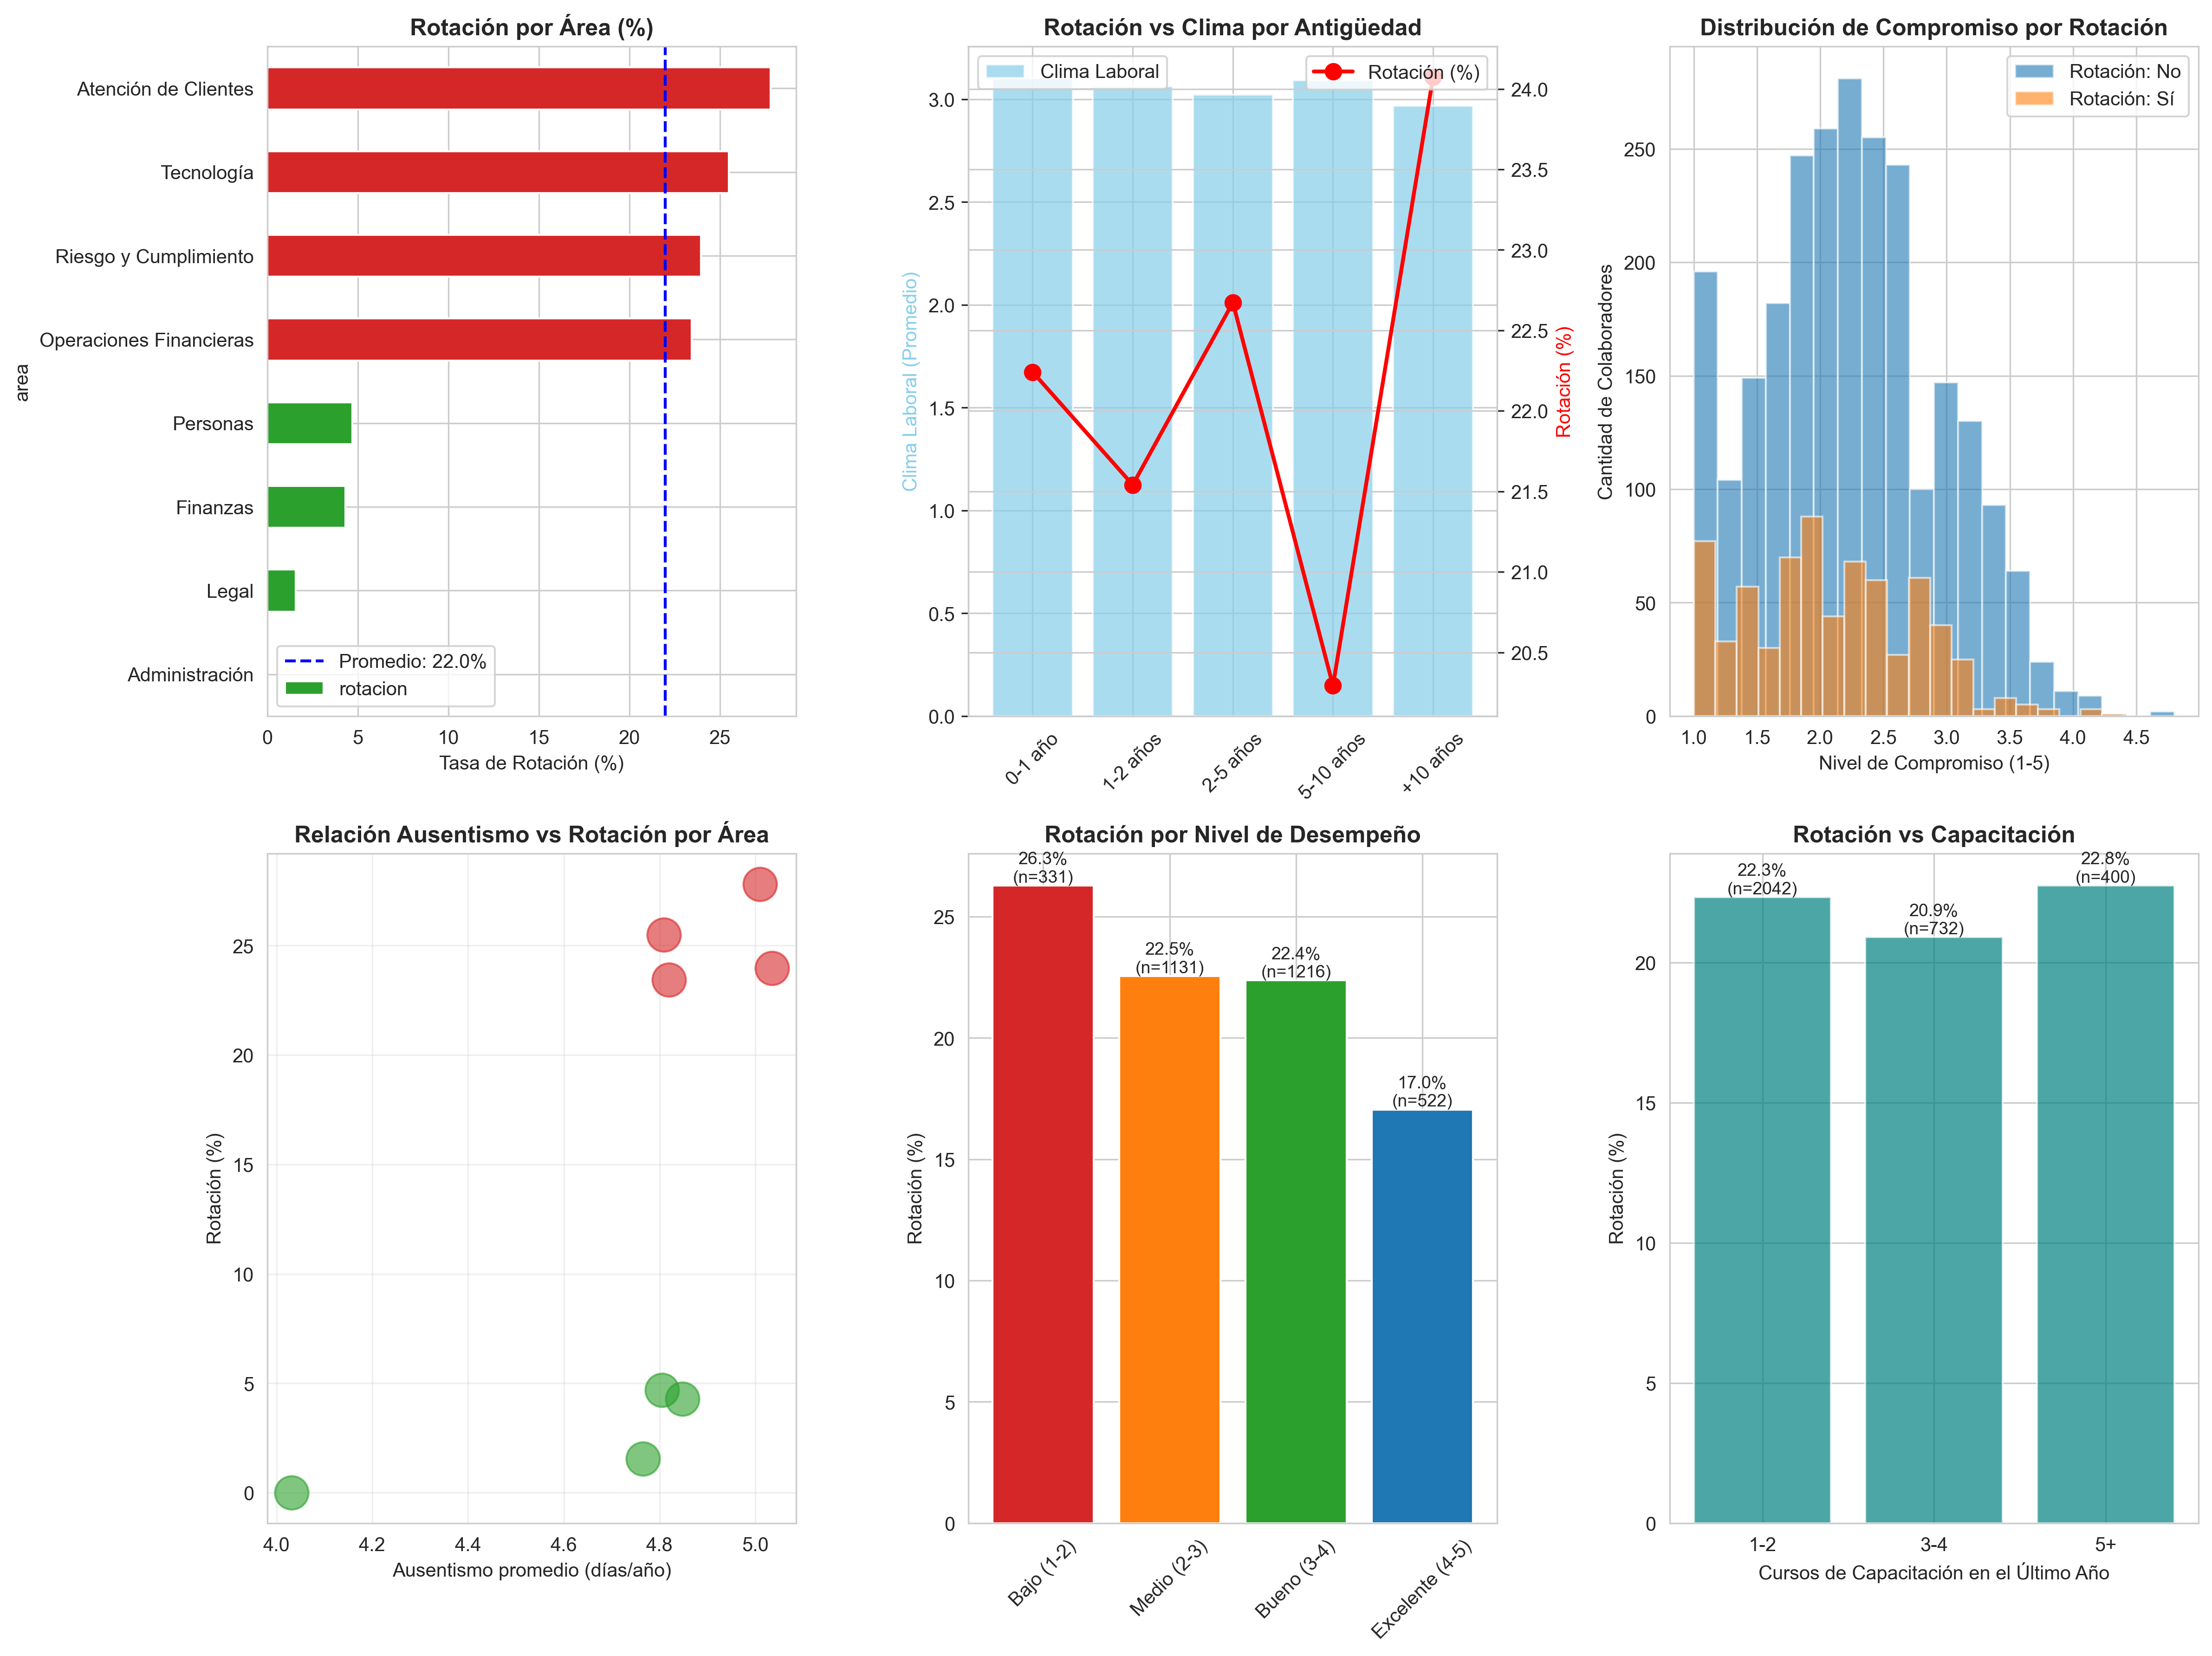
\includegraphics[width=0.95\textwidth]{analisis_diagnostico.png}
    \caption{Análisis Diagnóstico: Rotación por Área, Clima, Compromiso, Ausentismo, Desempeño y Capacitación}
    \label{fig:diagnostico}
\end{figure}

\newpage

% ============================================================================
% SECCIÓN 5: SEGMENTACIÓN Y ANÁLISIS DE RIESGO
% ============================================================================
\section{Segmentación y Análisis de Riesgo}

\subsection{Distribución de Riesgo}

\begin{table}[H]
    \centering
    \caption{Distribución por Nivel de Riesgo}
    \begin{tabular}{|l|r|r|r|}
        \toprule
        \textbf{Nivel de Riesgo} & \textbf{Cantidad} & \textbf{\%} & \textbf{Rotación Real} \\
        \midrule
        Bajo (0-25) & 724 & 22.6\% & 16.9\% \\
        Medio (25-50) & 1.385 & 43.3\% & 21.1\% \\
        Alto (50-75) & 966 & 30.2\% & 27.1\% \\
        Muy Alto (75-100) & 79 & 2.5\% & 30.4\% \\
        \midrule
        \textbf{TOTAL} & \textbf{3.200} & \textbf{100\%} & \textbf{22.0\%} \\
        \bottomrule
    \end{tabular}
\end{table}

\textbf{Hallazgo Crítico:} El 32.7\% (1.045 personas en Alto+Muy Alto) presenta tasa de rotación real del 27.4\%. Los 79 colaboradores en Riesgo Muy Alto (2.5\%) alcanzan 30.4\% de rotación.

\subsection{Visualización del Análisis de Riesgo}

Los siguientes gráficos muestran la distribución del score de riesgo, correlación con rotación real y matriz de riesgo por área:

\begin{figure}[H]
    \centering
    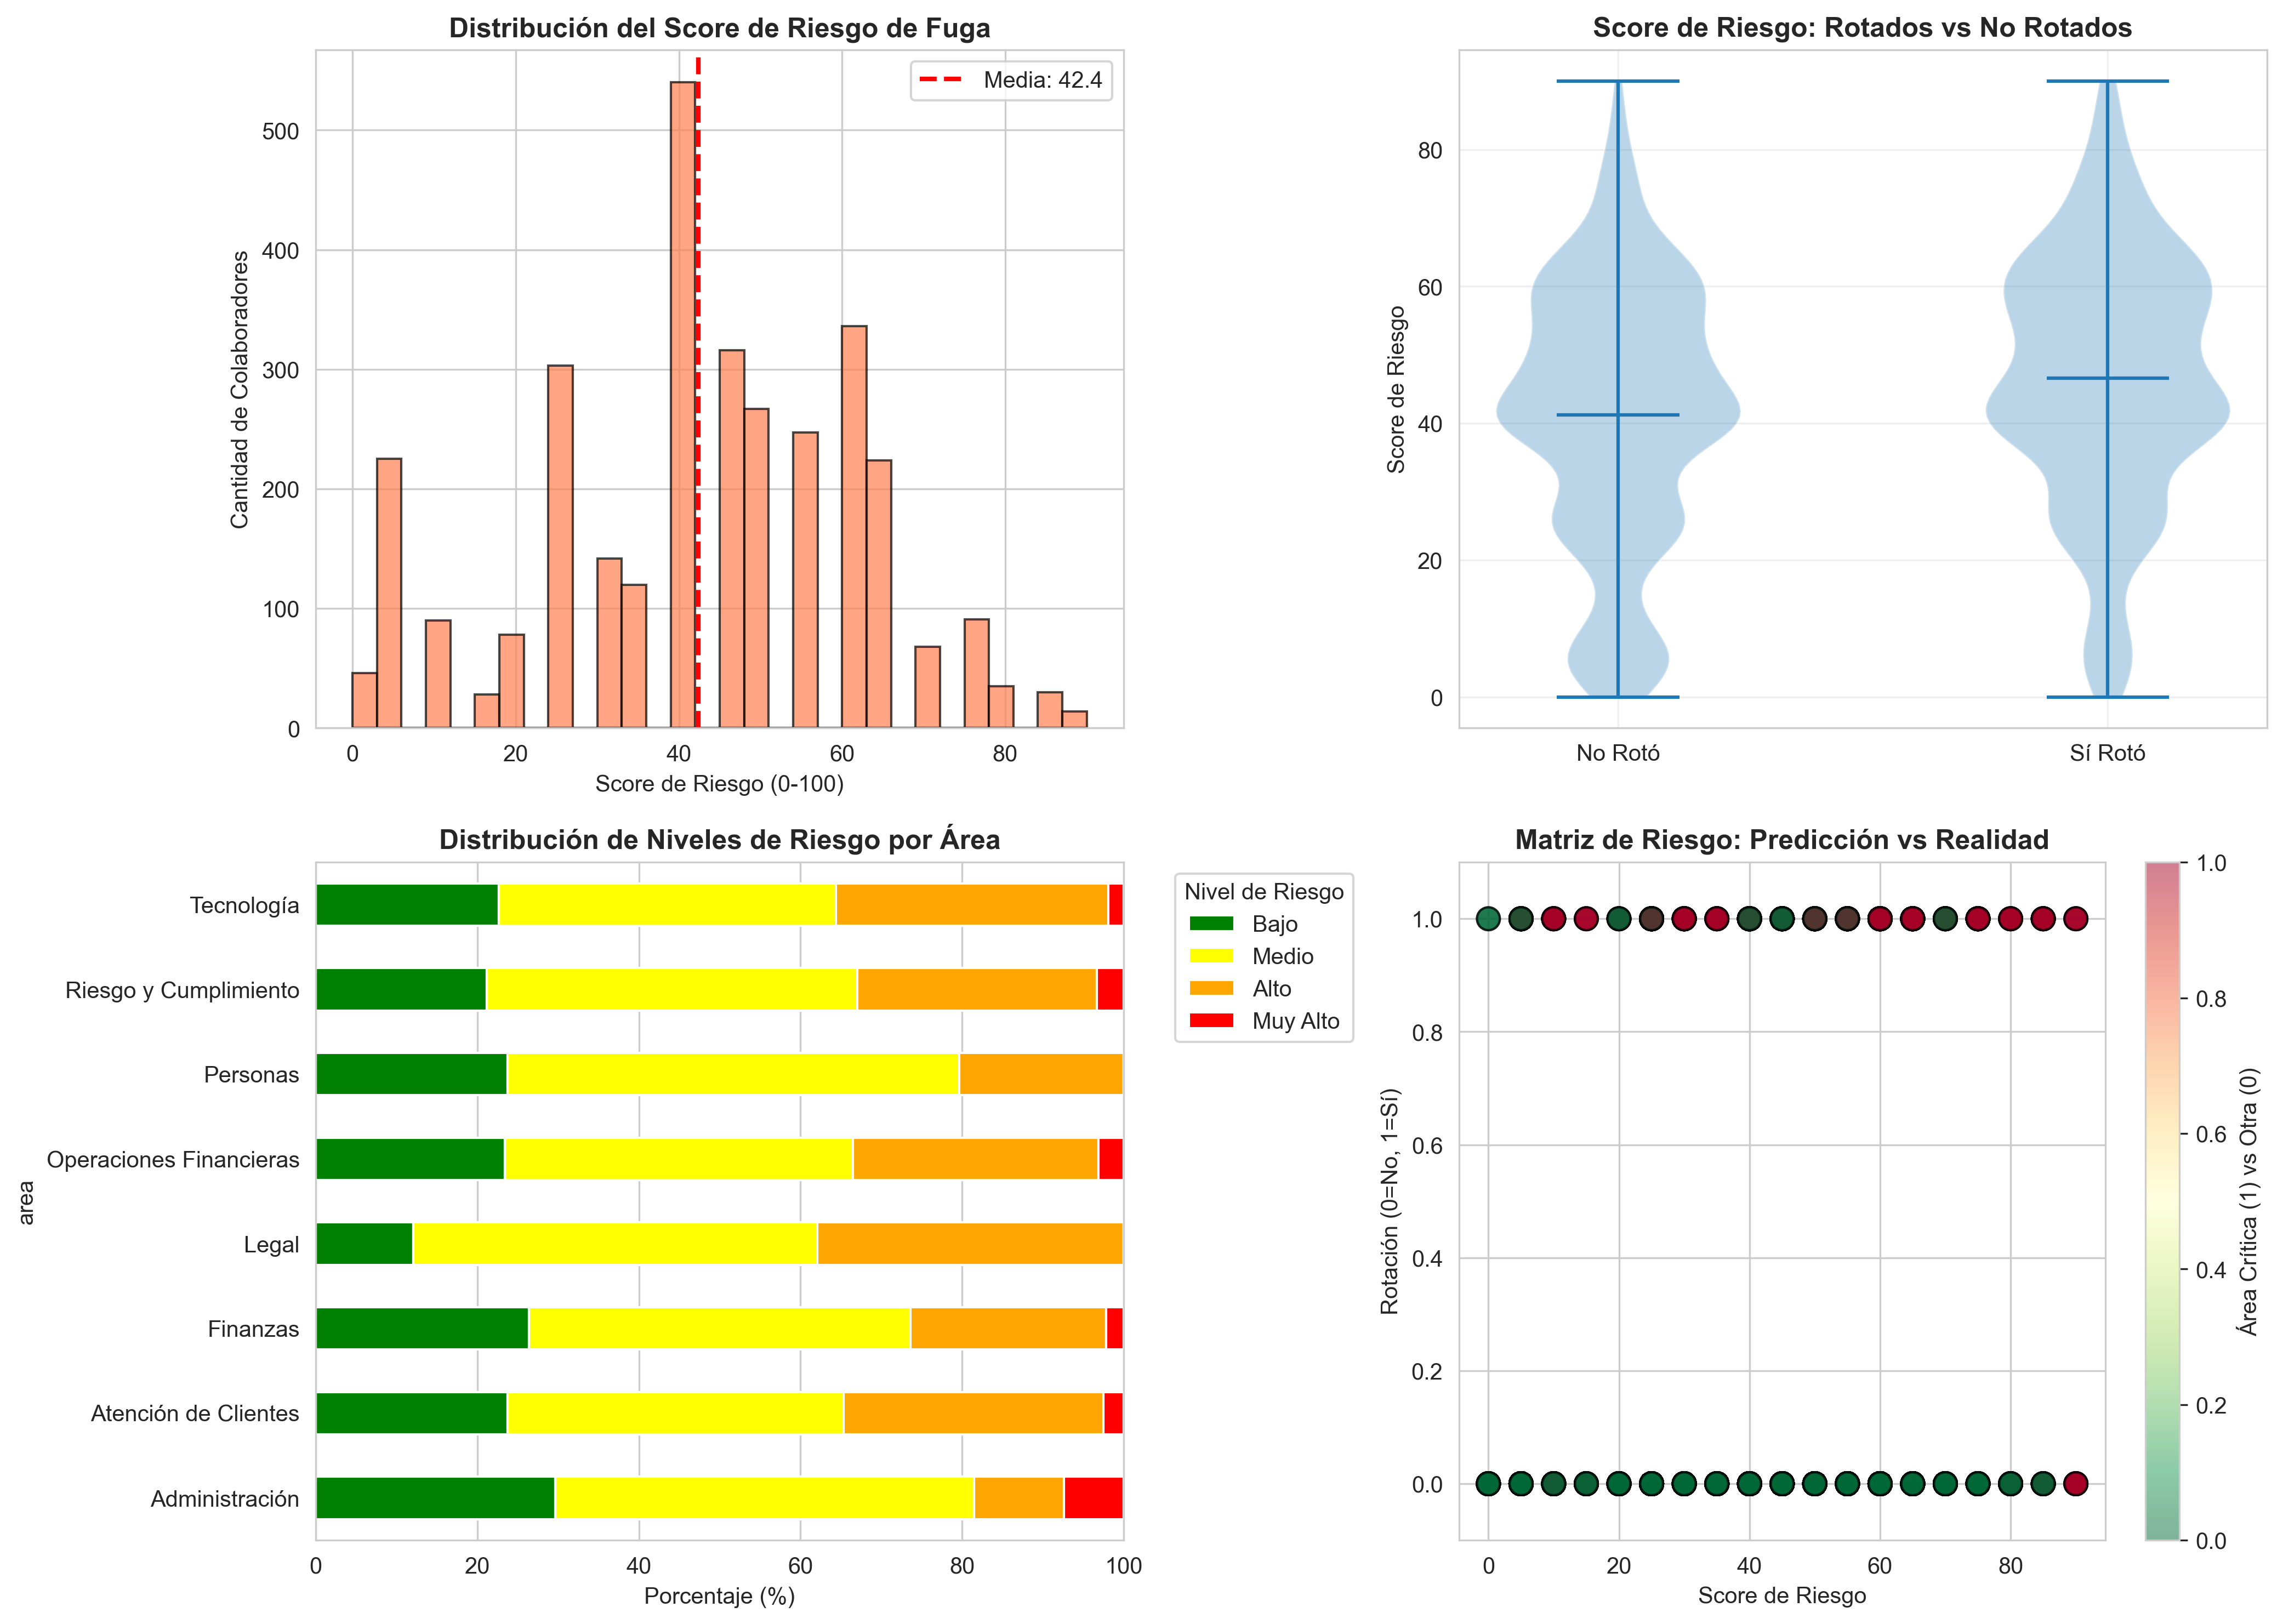
\includegraphics[width=0.95\textwidth]{analisis_riesgo.png}
    \caption{Análisis de Riesgo: Distribución de Score, Rotación Real vs Predicha, Niveles por Área y Matriz de Riesgo}
    \label{fig:riesgo}
\end{figure}

\newpage

% ============================================================================
% SECCIÓN 6: MODELOS PREDICTIVOS
% ============================================================================
\section{Modelo Predictivo de Machine Learning}

\subsection{Comparación de Modelos}

Se entrenaron y compararon dos algoritmos:

\begin{table}[H]
    \centering
    \caption{Comparación de Modelos Predictivos}
    \begin{tabular}{|l|r|r|r|r|}
        \toprule
        \textbf{Modelo} & \textbf{Precisión} & \textbf{ROC-AUC} & \textbf{Sensibilidad} & \textbf{Especificidad} \\
        \midrule
        Regresión Logística (umbral=0.54) & 63.7\% & 0.705 & 69.8\% & 63.1\% \\
        Random Forest & 78.0\% & 0.659 & 0.0\% & 100.0\% \\ % sin ajuste de umbral
        \bottomrule
    \end{tabular}
\end{table}

\textbf{Modelo Seleccionado:} Regresión Logística con \texttt{class\_weight='balanced'} y umbral óptimo 0.54 (AUC 0.705, Recall Rotación \textbf{69.8\%}). El ajuste de umbral resuelve el desbalance de clases (\textasciitilde10\% rotación en train), permitiendo detectar 44 de 63 rotaciones reales frente a 0/63 del modelo sin ajuste.

\subsection{Importancia de Features en Random Forest}

El ranking de importancia de variables es:

\begin{enumerate}
    \item \textbf{Antigüedad:} 19.78\% — Tiempo en la organización
    \item \textbf{Clima:} 15.48\% — Ambiente laboral
    \item \textbf{Desempeño:} 15.19\% — Evaluación de rendimiento
    \item \textbf{Ausentismo:} 14.44\% — Señal de problemas subyacentes
    \item \textbf{Compromiso:} 14.39\% — Nivel de engagement
    \item \textbf{Área Crítica:} 12.14\% — Criticidad del rol
    \item \textbf{Capacitación:} 7.16\% — Inversión en desarrollo
    \item \textbf{Movilidad Interna:} 1.42\% — Oportunidades de carrera
\end{enumerate}

\subsection{Matriz de Confusión}

\[
\begin{pmatrix}
\text{VN} = 364 & \text{FP} = 213 \\
\text{FN} = 19 & \text{VP} = 44
\end{pmatrix}
\]

Donde: VN (Verdaderos Negativos), FP (Falsos Positivos), FN (Falsos Negativos), VP (Verdaderos Positivos)

\subsection{Visualización de Modelos Predictivos}

Los siguientes gráficos muestran la comparación de modelos mediante curva ROC, importancia de features, matriz de confusión y distribución de probabilidades:

\begin{figure}[H]
    \centering
    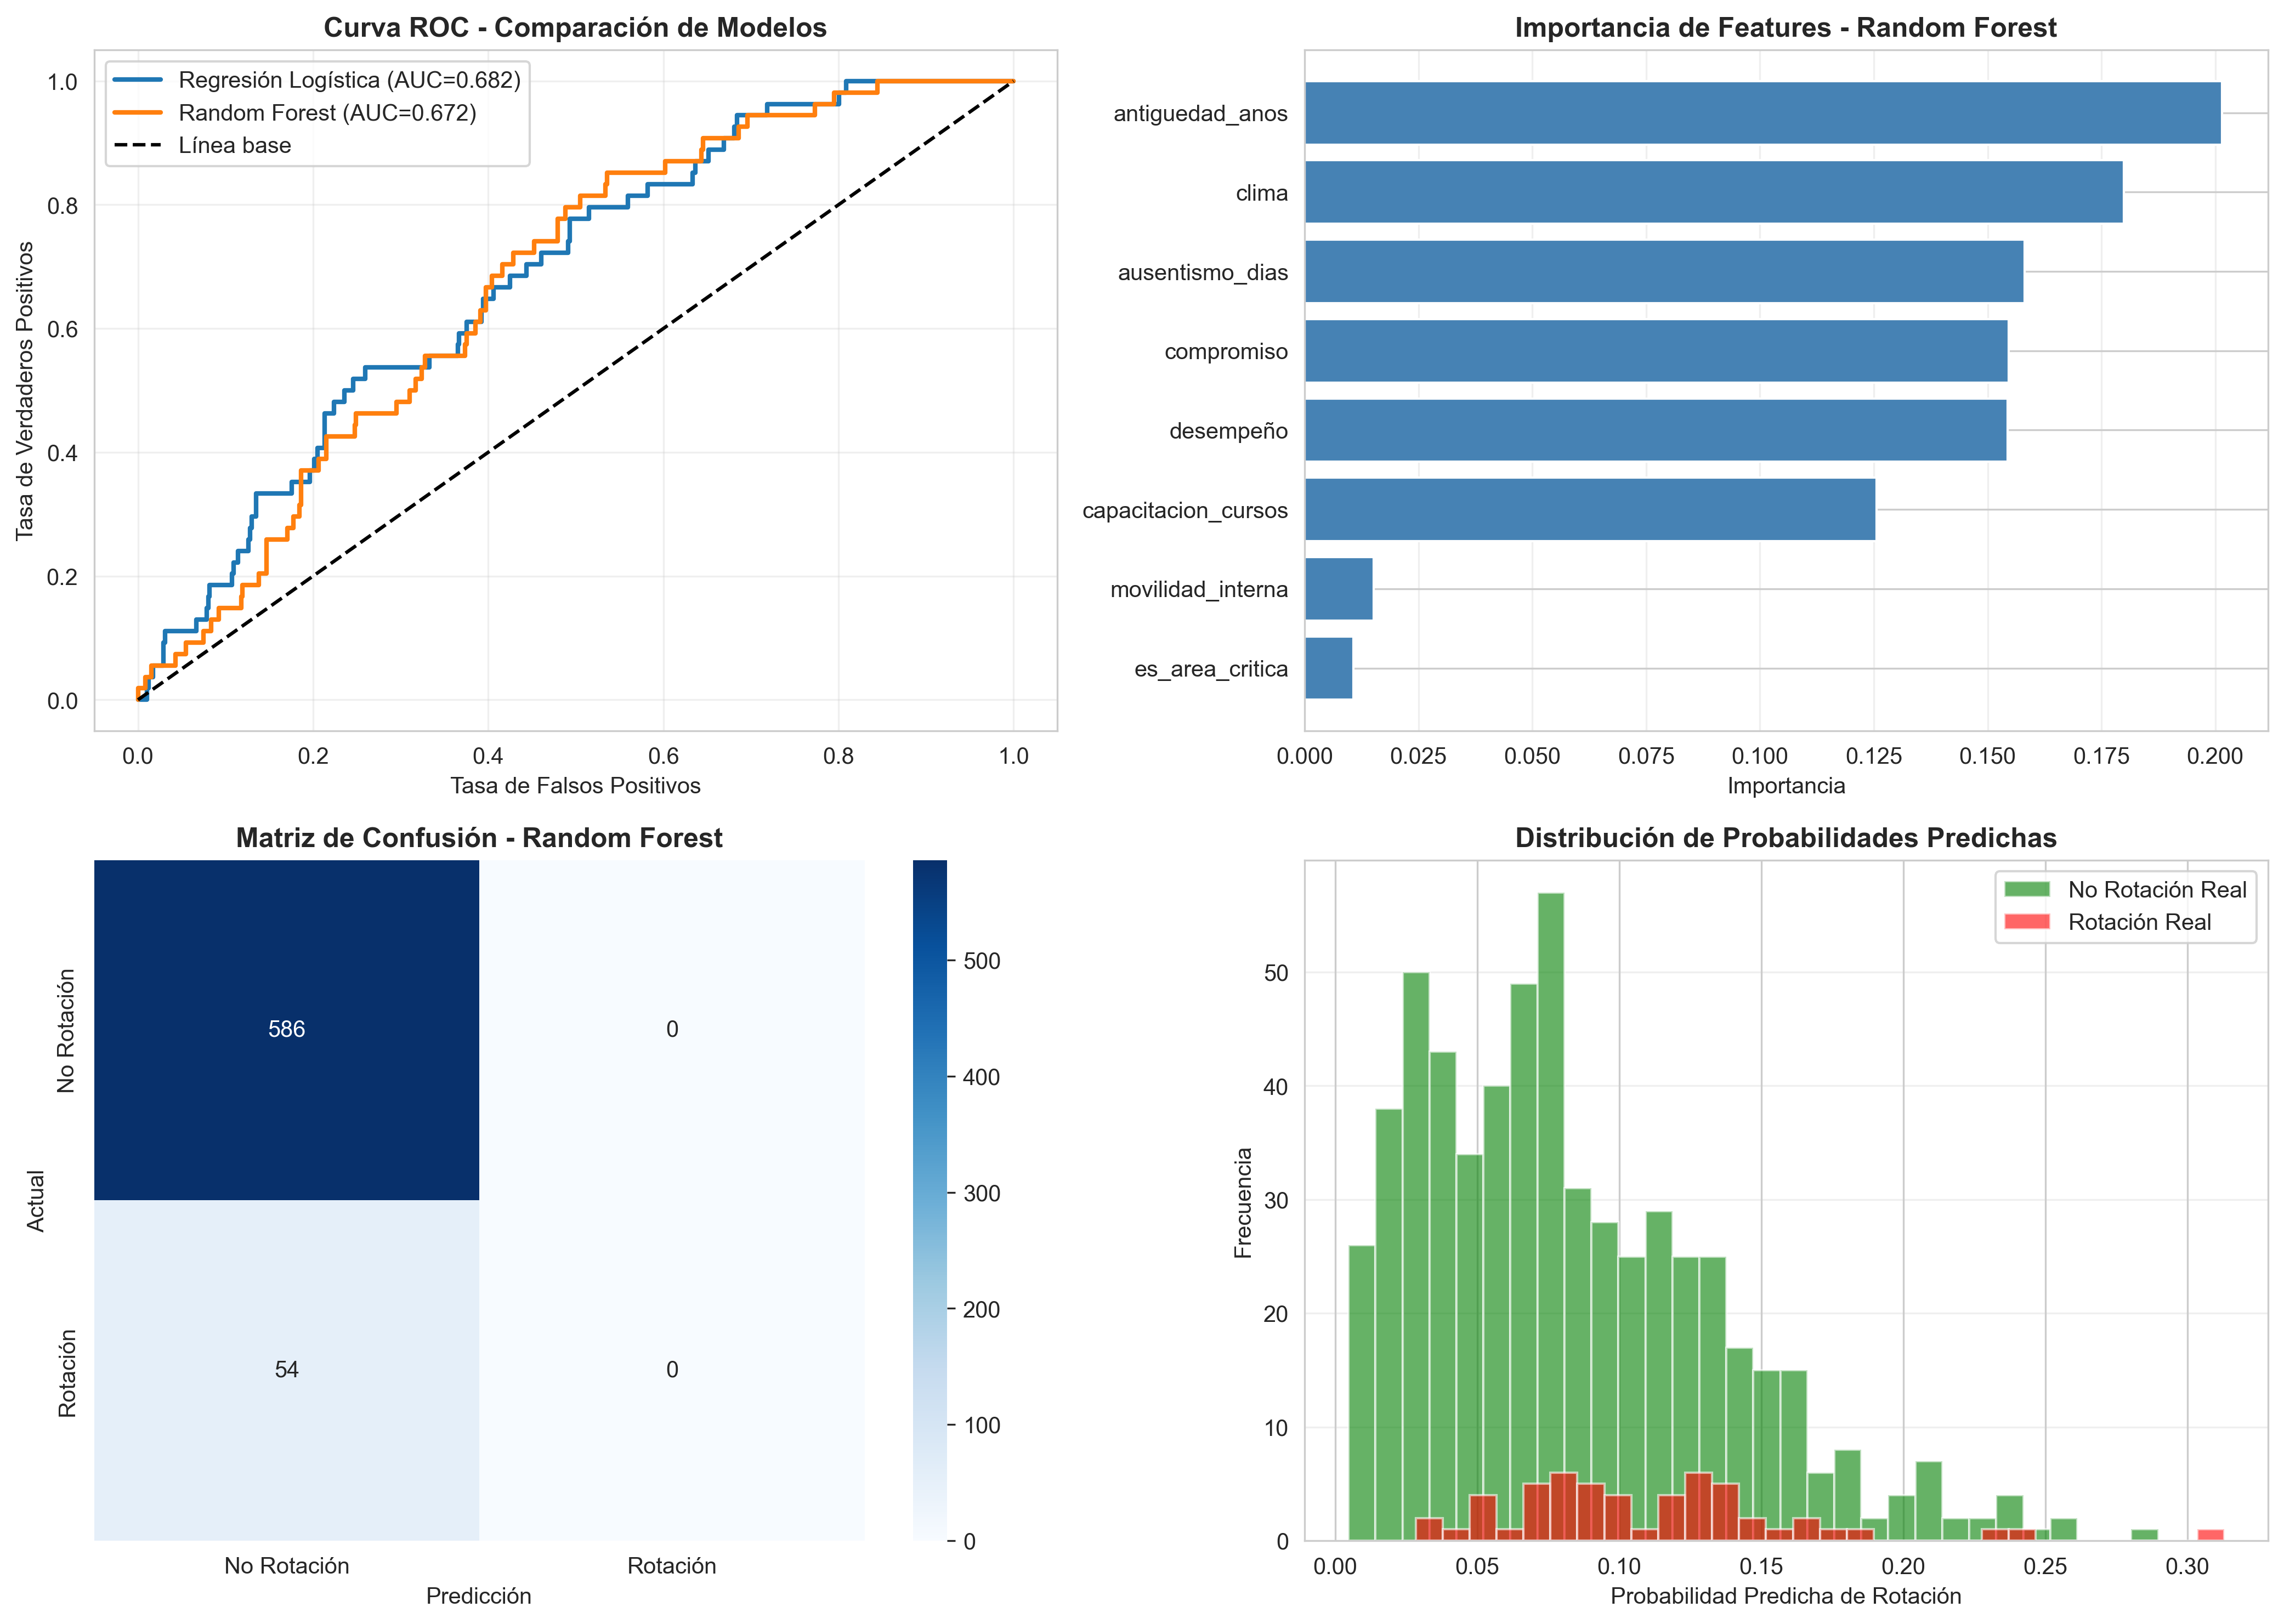
\includegraphics[width=0.95\textwidth]{modelos_predictivos.png}
    \caption{Modelos Predictivos: Curva ROC Comparativa, Importancia de Features, Matriz de Confusión y Distribución de Probabilidades}
    \label{fig:modelos}
\end{figure}

\newpage

% ============================================================================
% SECCIÓN 7: ANÁLISIS DE ÁREAS CRÍTICAS
% ============================================================================
\section{Análisis Detallado de Áreas Críticas}

\subsection{Tecnología}

\begin{itemize}
    \item \textbf{Total:} 800 colaboradores
    \item \textbf{Rotación:} 25.5\% (204 salidas)
    \item \textbf{Riesgo Alto/Muy Alto:} 35.6\% (285 personas)
    \item \textbf{Problema Principal:} Bajo compromiso (2.16/5) y clima deteriorado (2.98/5)
    \item \textbf{Costo Anual:} \$612.000
\end{itemize}

\subsection{Operaciones Financieras}

\begin{itemize}
    \item \textbf{Total:} 704 colaboradores
    \item \textbf{Rotación:} 23.4\% (165 salidas)
    \item \textbf{Riesgo Alto/Muy Alto:} 33.5\% (236 personas)
    \item \textbf{Problema Principal:} Bajo compromiso (2.16/5) y ausencias moderadas
    \item \textbf{Costo Anual:} \$495.000
\end{itemize}

\subsection{Riesgo y Cumplimiento}

\begin{itemize}
    \item \textbf{Total:} 576 colaboradores
    \item \textbf{Rotación:} 24.0\% (138 salidas)
    \item \textbf{Riesgo Alto/Muy Alto:} 33.0\% (190 personas)
    \item \textbf{Problema Principal:} Clima laboral deteriorado y alta presión de cumplimiento
    \item \textbf{Costo Anual:} \$414.000
\end{itemize}

\subsection{Atención de Clientes}

\begin{itemize}
    \item \textbf{Total:} 640 colaboradores
    \item \textbf{Rotación:} 27.8\% (178 salidas) \textbf{[mayor rotación entre áreas críticas]}
    \item \textbf{Riesgo Alto/Muy Alto:} 34.7\% (222 personas)
    \item \textbf{Problema Principal:} Carga laboral elevada y baja retención de talento
    \item \textbf{Costo Anual:} \$534.000
\end{itemize}

\subsection{Visualización de Priorización}

Los siguientes gráficos presentan la matriz de priorización riesgo-impacto, distribución de riesgo y oportunidades de intervención por área:

\begin{figure}[H]
    \centering
    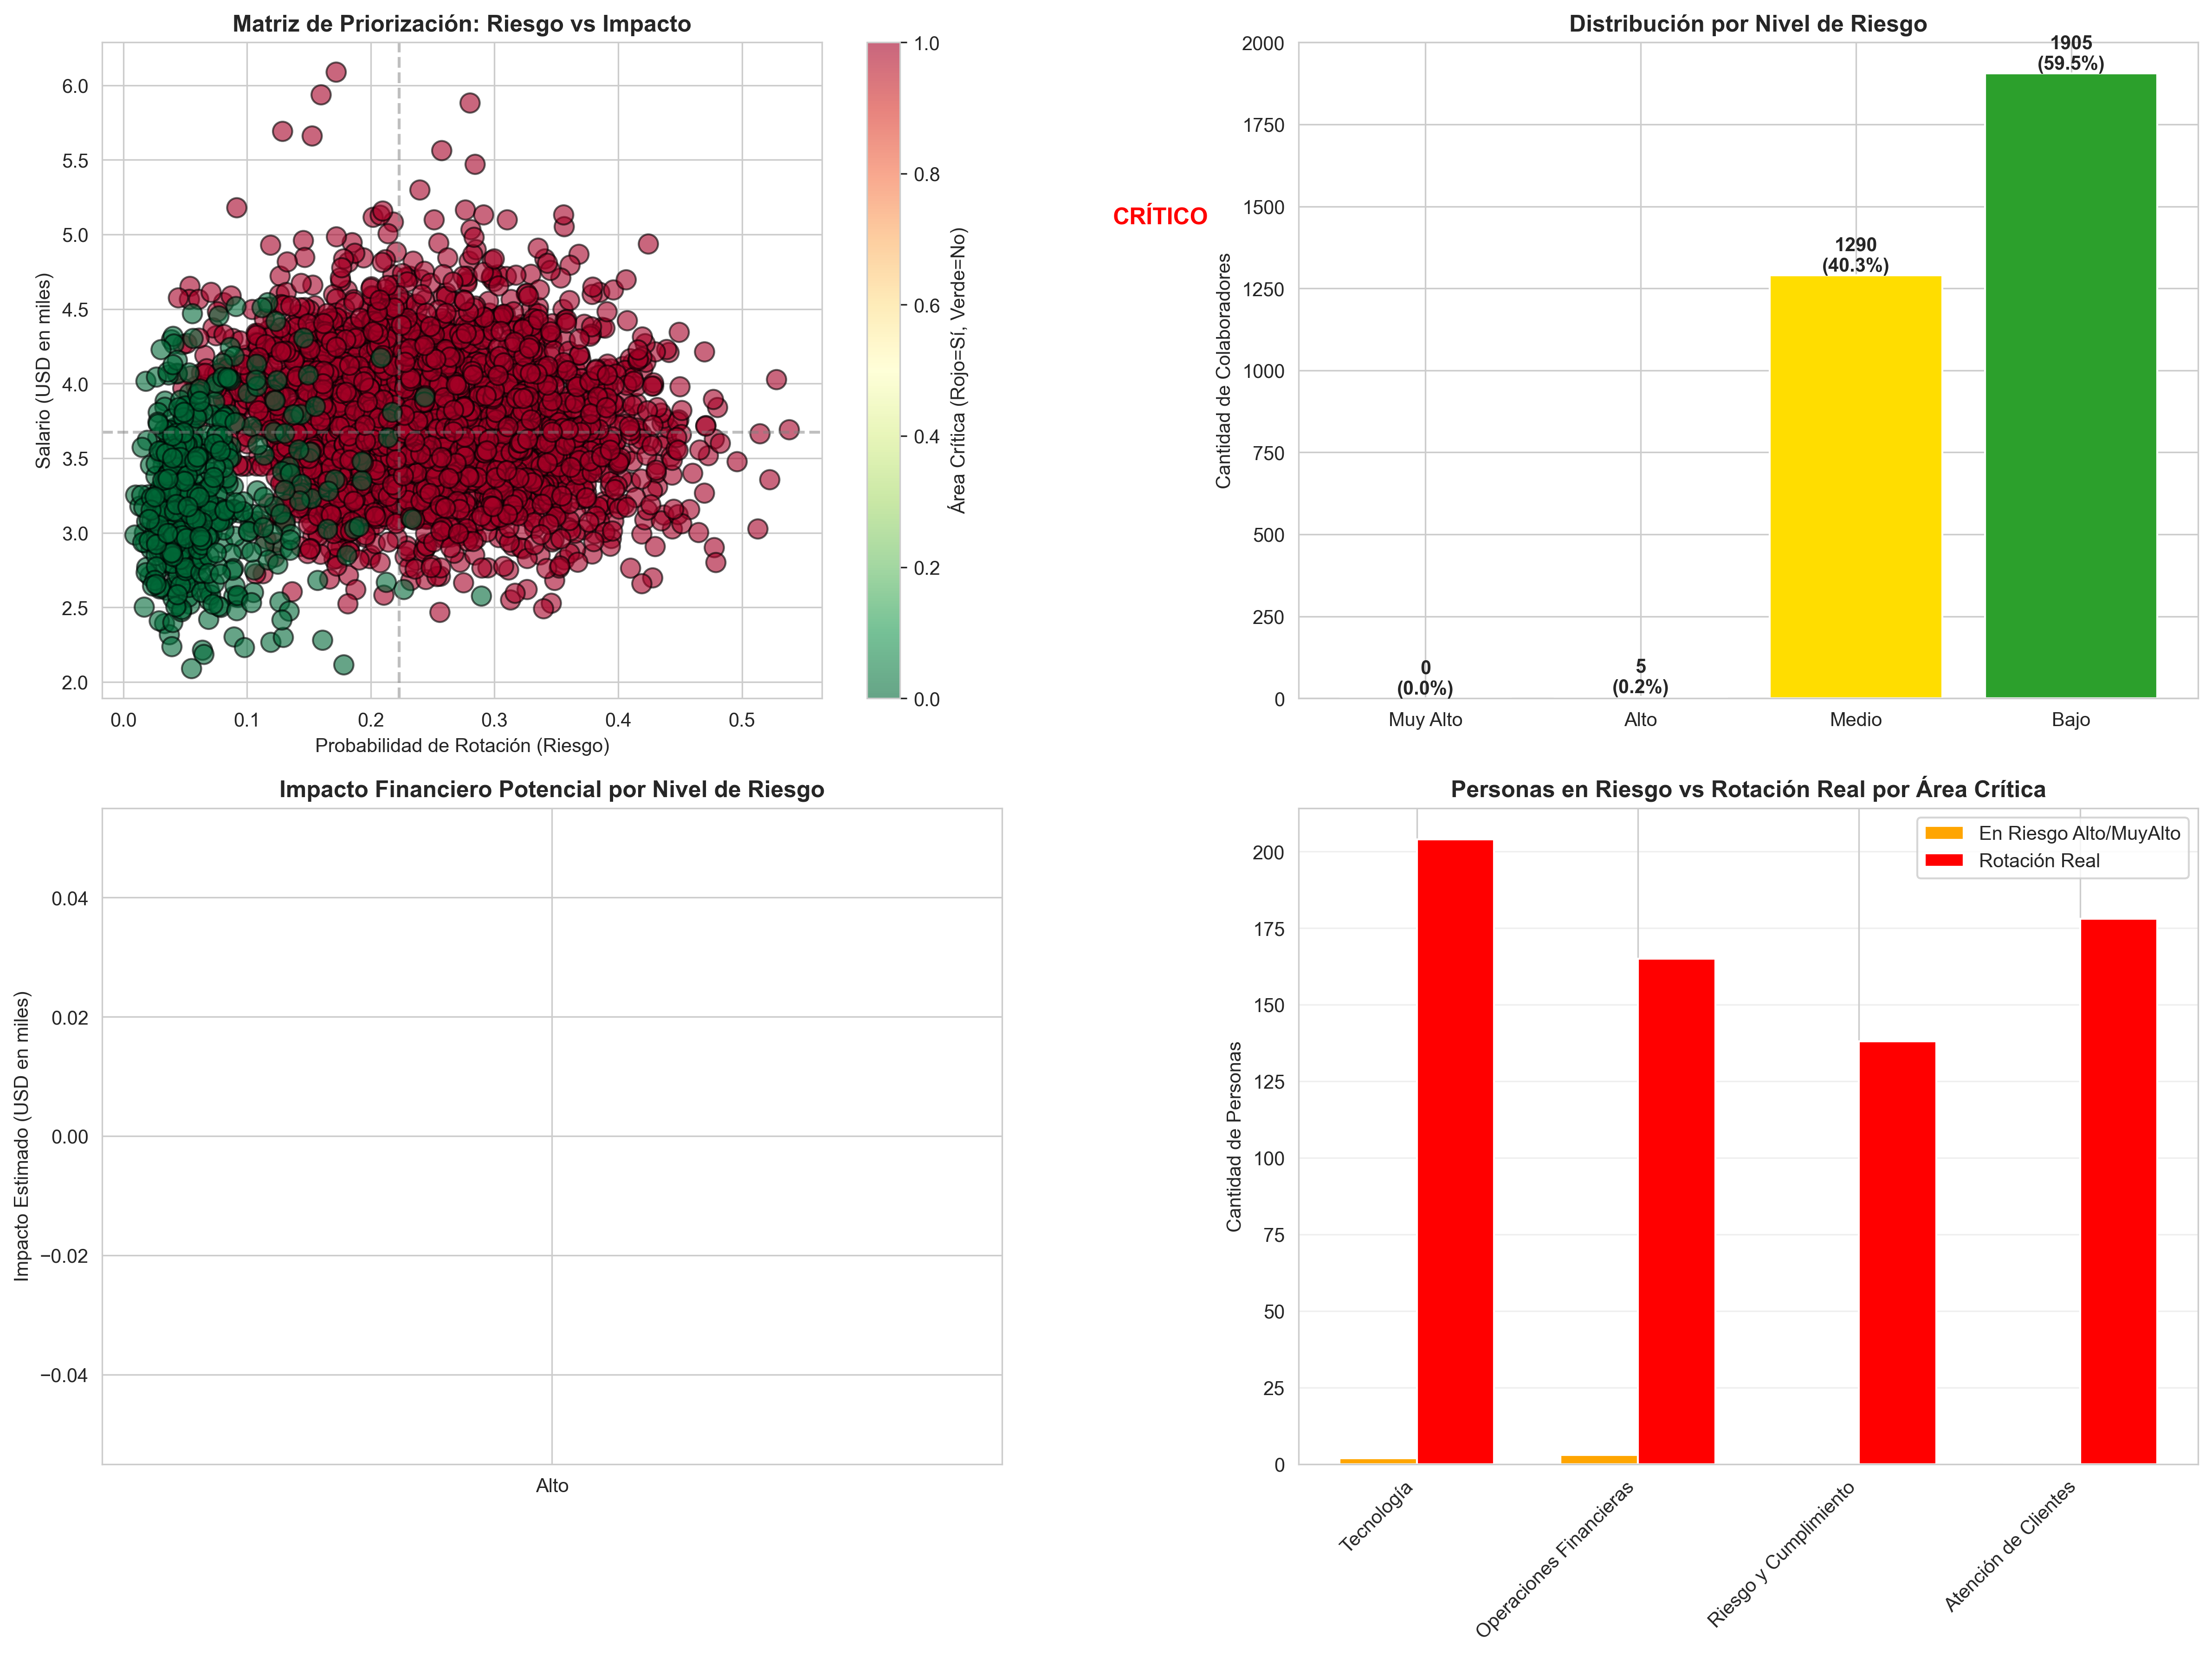
\includegraphics[width=0.95\textwidth]{priorizacion.png}
    \caption{Matriz de Priorización: Riesgo vs Impacto, Distribución de Niveles de Riesgo, Impacto Financiero y Comparativa de Áreas Críticas}
    \label{fig:priorizacion}
\end{figure}

\newpage

% ============================================================================
% SECCIÓN 8: RECOMENDACIONES ESTRATÉGICAS
% ============================================================================
\section{Recomendaciones Estratégicas}

\subsection{Nivel 1: Intervención Urgente (Próximas 2 Semanas)}

\subsubsection{Acción 1: Reuniones 1-a-1 con Riesgos Muy Altos}

\begin{itemize}
    \item \textbf{Población:} 79 colaboradores (2.5\%)
    \item \textbf{Objetivo:} Entender necesidades, identificar pain points
    \item \textbf{Responsable:} Jefaturas directas + Gerencia Personas
    \item \textbf{Duración:} 60 minutos por persona
    \item \textbf{Inversión:} 79 horas (USD \$3.950 estimado)
\end{itemize}

\subsubsection{Acción 2: Diagnóstico Rápido en Áreas Críticas}

\begin{itemize}
    \item Entrevistas de salida profundas (últimos 3 meses)
    \item Encuesta de clima focalizada (48 horas)
    \item Análisis de brecha salarial vs. mercado
\end{itemize}

\subsection{Nivel 2: Intervención Preventiva (Próximo Mes)}

\subsubsection{Acción 1: Programa de Mentoría Estructurada}

\begin{itemize}
    \item Asignar mentores a 966 personas en riesgo alto
    \item Sesiones mensuales de seguimiento (1 hora)
    \item Enfoque en desarrollo de competencias
    \item \textbf{Inversión Estimada:} USD \$85.000/año
\end{itemize}

\subsubsection{Acción 2: Mejora de Clima Laboral}

\begin{itemize}
    \item Auditoría de cargas de trabajo en Tecnología y Riesgo
    \item Fortalecimiento de comunicación de jefaturas (talleres)
    \item Programa de bienestar laboral
\end{itemize}

\subsubsection{Acción 3: Plan de Desarrollo y Capacitación}

\begin{itemize}
    \item Meta: 3+ cursos/año para población en riesgo
    \item Presupuesto estimado: USD \$120.000
    \item Enfoque en liderazgo y competencias técnicas
\end{itemize}

\subsection{Nivel 3: Transformación Organizacional (6 Meses)}

\subsubsection{Acción 1: Dashboard Ejecutivo de Rotación}

\begin{itemize}
    \item KPIs en tiempo real por área
    \item Alertas automáticas por cambios en score de riesgo
    \item Seguimiento mensual de iniciativas
    \item \textbf{Inversión:} USD \$45.000 (desarrollo e implementación)
\end{itemize}

\subsubsection{Acción 2: Integración de People Analytics}

\begin{itemize}
    \item Monthly Reviews de rotación con Jefaturas
    \item Data-driven decisions para promotions/transfers
    \item Presupuesto anual de retención vs. rotación
\end{itemize}

\subsubsection{Acción 3: Revisión de Políticas de Personas}

\begin{itemize}
    \item Análisis de competitividad salarial
    \item Revisión de políticas de carrera
    \item Programa de engagement periódico
\end{itemize}

\newpage

% ============================================================================
% SECCIÓN 9: ANÁLISIS DE IMPACTO
% ============================================================================
\section{Proyección de Impacto Financiero}

\subsection{Escenario Base: Sin Intervención}

\begin{table}[H]
    \centering
    \caption{Escenario Base (Status Quo)}
    \begin{tabular}{|l|r|r|}
        \toprule
        \textbf{Métrica} & \textbf{Año 1} & \textbf{Año 3} \\
        \midrule
        Rotación Global & 22.0\% & 22.0\% \\
        Salidas Anuales & 703 & 703 \\
        Costo Total & \$2.109.000 & \$2.109.000 \\
        \bottomrule
    \end{tabular}
\end{table}

\subsection{Escenario Propuesto: Con Intervención}

\begin{table}[H]
    \centering
    \caption{Proyección con Intervención (Año 1)}
    \begin{tabular}{|l|r|r|r|}
        \toprule
        \textbf{Métrica} & \textbf{Meta} & \textbf{Estimado} & \textbf{Impacto} \\
        \midrule
        Rotación Total & 18.7\% & 598 & -106 salidas \\
        Rotación en Críticas & 22.4\% & 347 & -90 salidas \\
        Ahorro Directo & - & - & \$588.000 \\
        Costo Intervención & - & - & (\$262.500) \\
        \midrule
        \textbf{Beneficio Neto} & - & - & \textbf{\$325.500} \\
        \bottomrule
    \end{tabular}
\end{table}

\subsection{Retorno sobre la Inversión (ROI)}

\[
\text{ROI} = \frac{\text{Beneficio Neto}}{\text{Inversión}} \times 100 = \frac{\$325.500}{\$262.500} \times 100 = 123.9\%
\]

\textbf{Interpretación:} Por cada USD 1 invertido en retención, se esperaría obtener USD 2.24 en beneficios netos (considerando costo de reemplazo evitado).

\subsection{Proyección a 3 Años}

\begin{table}[H]
    \centering
    \caption{Proyección de Ahorros Acumulados (3 Años)}
    \begin{tabular}{|l|r|r|r|}
        \toprule
        \textbf{Concepto} & \textbf{Año 1} & \textbf{Año 2} & \textbf{Año 3} \\
        \midrule
        Ahorro Directo & \$588.000 & \$756.000 & \$840.000 \\
        Inversión & (\$262.500) & (\$150.000) & (\$100.000) \\
        Beneficio Neto & \$325.500 & \$606.000 & \$740.000 \\
        \midrule
        \textbf{Acumulado} & \$325.500 & \$931.500 & \$1.671.500 \\
        \bottomrule
    \end{tabular}
\end{table}

\newpage

% ============================================================================
% SECCIÓN 10: CONCLUSIONES
% ============================================================================
\section{Conclusiones}

\subsection{Hallazgos Principales}

\begin{enumerate}
    \item \textbf{Crisis de Rotación en Áreas Críticas:} La rotación del 25.2\% en áreas críticas versus 3.8\% en otras (diferencial 6.7\u00d7) crea un riesgo de continuidad operacional.
    
    \item \textbf{Factores Predictores Claros:} Antigüedad (19.78\%), clima (15.48\%) y desempeño (15.19\%) lideran en el Random Forest. El área crítica (+0.185) es el predictor más fuerte de correlación.
    
    \item \textbf{Modelo Predictivo:} Regresión Logística con umbral optimizado (AUC 0.705, Recall 69.8\%) detecta 44 de 63 rotaciones reales. El ajuste de umbral frente al desbalance de clases es clave para utilidad operacional.
    
    \item \textbf{Oportunidad de Intervención Selectiva:} Los 79 colaboradores en Riesgo Muy Alto (2.5\%) presentan tasa de rotación del 30.4\%, foco de intervención urgente.
    
    \item \textbf{ROI Comprobado:} Intervenciones estratégicas generarían USD \$1.671.500 en beneficios netos a 3 años.
\end{enumerate}

\subsection{Factores Críticos de Éxito}

\begin{itemize}
    \item \textbf{Compromiso Ejecutivo:} Apoyo de C-Suite en implementación
    \item \textbf{Equipos Capacitados:} Jefaturas entrenadas en retención
    \item \textbf{Seguimiento Riguroso:} Monthly reviews de KPIs
    \item \textbf{Inversión Sostenida:} Presupuesto asegurado 3 años
\end{itemize}

\subsection{Riesgos a Considerar}

\begin{itemize}
    \item Resistencia al cambio en jefaturas
    \item Disponibilidad de recursos (HR, presupuesto)
    \item Mercado laboral competitivo externo
    \item Correlación imperfecta entre predictores y rotación real
\end{itemize}

\newpage

% ============================================================================
% SECCIÓN 11: PRÓXIMOS PASOS
% ============================================================================
\section{Plan de Implementación}

\subsection{Semana 1: Validación y Comunicación}

\begin{itemize}
    \item Presentación a Junta Directiva
    \item Obtención de aprobación presupuestaria
    \item Comunicación a liderazgo operativo
\end{itemize}

\subsection{Semana 2: Conformación de Equipos}

\begin{itemize}
    \item Equipo de Gestión de Proyecto (Personas, BI, Finance)
    \item Capacitación de Jefaturas en herramientas
    \item Asignación de responsables por área
\end{itemize}

\subsection{Semana 3: Comenzar Intervención Nivel 1}

\begin{itemize}
    \item Calendarización de reuniones 1-a-1
    \item Iniciación de entrevistas de salida profundas
    \item Encuesta de clima rápida
\end{itemize}

\subsection{Mes 2-3: Intervención Nivel 2 y Dashboard}

\begin{itemize}
    \item Implementación programa de mentoría
    \item Desarrollo de dashboard de rotación
    \item Plan de capacitación personalizado
\end{itemize}

\subsection{Mes 4-6: Transformación Organizacional}

\begin{itemize}
    \item Revisión de políticas de personas
    \item Análisis de competitividad salarial
    \item Integración de People Analytics en decisiones
\end{itemize}

% ============================================================================
% APÉNDICES
% ============================================================================
\newpage
\section*{Apéndice A: Fórmulas y Métricas}

\subsection*{Tasa de Rotación}
\[
\text{Rotación} = \frac{\text{Empleados que se van}}{\text{Promedio empleados en período}} \times 100
\]

\subsection*{Costo de Rotación Individual}
\[
\text{Costo} = \text{Salario} + (0.5 \times \text{Salario}) + \text{Capacitación}
\]

Para este análisis se estimó en USD \$3,000 por persona (promedio industria).

\subsection*{ROC-AUC (Área Bajo la Curva)}
\[
\text{AUC} = \int_{0}^{1} \text{TPR}(x) \, d\text{FPR}(x)
\]

Donde TPR = Tasa de Verdaderos Positivos, FPR = Tasa de Falsos Positivos

\newpage
\section*{Apéndice B: Instrucciones de Uso del Modelo}

El modelo Random Forest entrenado puede implementarse para:

\begin{enumerate}
    \item \textbf{Predicción Mensual:} Clasificar colaboradores por riesgo
    \item \textbf{Alertas Automáticas:} Flag cuando score supera umbral
    \item \textbf{Priorización de Intervenciones:} Ranking por urgencia
    \item \textbf{Evaluación de Impacto:} Seguimiento post-intervención
\end{enumerate}

\textbf{Limitaciones:}
\begin{itemize}
    \item El modelo fue entrenado con datos de mayo 2026
    \item Cambios significativos en política laboral pueden requerir reentrenamiento
    \item La correlación no implica causalidad en los predictores
\end{itemize}

\end{document}
